\documentclass{beamer}
\usepackage[utf8x]{inputenc}
\usepackage{default}
\usepackage{verbatim}
\newcommand{\Ardrone}{Ar Drone$^{\copyright}$ }

\title{Autonomous Flight With the \Ardrone drone}
\author{Maarten Inja and Maarten de Waard}
\institute{UvA}
\usetheme{Warsaw}
\newcommand{\slide}[2]
{
\begin{frame}
\begin{block}{#1} 

#2

\end{block} \end{frame}
}



\begin{document}
\begin{frame}
\titlepage
\end{frame}



% wat is de ardrone?
% wat willen we er mee doen?
% hoe gaan we dat doen?
% 
% wat is allemaal gelukt?


\section{Introduction}
\slide{The \Ardrone}{
The \Ardrone is an over WiFi remote controlled quadrocopter that has several onboard sensors:
\begin{itemize}
	\item One vertical camera, pointing downwards
	\item One horizontal camera, pointing forward 
	\item Ultrasound altimeter, to measure the altitude
    \item 3 axis accelerometer (measures propellor acceleration)
    \item 2 axis gyrometer 
    \item 1 yaw precision gyrometer
\end{itemize}
Furthermore, it has an onboard computer system running Linux. 

% PROP HIER PLAATJES VAN DE AR DRONE

}

\begin{frame}
\frametitle{Movement Angles}

  \begin{picture}(0.0,0.0) 
     \put(80.0,-100.0){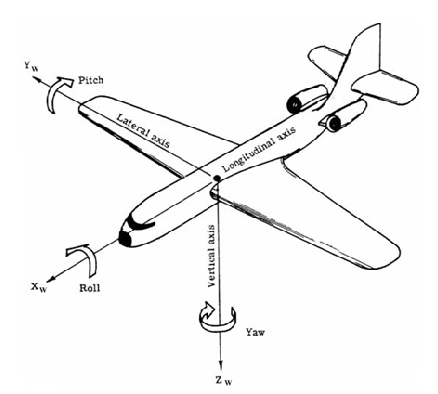
\includegraphics[width=0.5\textwidth]{pitchYawRoll.png}}
  \end{picture}
\end{frame}



\slide{Our Goal}{
Summer-IMAV 2011 Indoor competition, some sub-tasks of the exploration challenge:
\begin{itemize}
    \item Pick-up Object
    \item Exit Building
    \item Release Object
\end{itemize}

% PROP HIER DAT PLAATJE BIJ VAN DE SETTING
}

\section{How it's done}
\slide{Controlling The Drone}{
\begin{itemize}
    \item Direct Control
        \begin{itemize}
            \item Sending AT-Commands to ports
            \item Listening on different ports to decode navigation data and video
        \end{itemize}
    \item SDK, the Software Development Kit
        \begin{itemize}
            \item A complete framework that takes care of decoding and encoding
            \item Over complicated
            \item Othermans work
        \end{itemize}
    \item Extending C with Python
        \begin{itemize}
            \item We are better at Python
            \item Python is less complicated 
        \end{itemize}
\end{itemize}
}

\slide{Finding The Object}{
To find the object the drone complete a search pattern
\begin{itemize}
    \item Go to altitude X
    \item Rotate 360 degrees
    \item If the object has not been found, increase altitude X and repeat
\end{itemize}
}

\slide{Recognizing The Object}{
\begin{itemize}
    \item Convert video frame to HSV
    \item Discard pixels that do not match the color of the object
    \item Template match to find the middle of the object
    \item Calculate the distance by calculating the amount of recognized pixels
\end{itemize}
% example of such a frame
}

\slide{Pick Up The Object}{
\begin{itemize}
    \item Get the object in the middle of the screen
    \item Fly towards the object
    \item Hover in front of the object at a distance of 0.5 metres 
    \item Fly above the object to pick it up
\end{itemize}
We send variable steering commands to the \Ardrone, depending on the distance of the object and its location in the image to first radically steer in the right direction and then presicely center the object.
}


\section{Problems \& Solutions}
\slide{Problems}{
\begin{itemize}
    \item Flying errors
    \item Object weight
    \item Pick-up method
\end{itemize}
}

\slide{Unsuccesful Explored Options}{
\begin{itemize}
    \item Detect unwanted movements and steer against those
    \item Flat-trim at the start of each run
\end{itemize}
}

\slide{Solutions}{
\begin{itemize}
    \item A floor with texture; put random things on the floor 
    \item Restart when the flying error is too big
    \item Bigger object and hook
\end{itemize}
}


\section{Results}
\slide{Results}{
We can show you a replay and a movie of a succesful pick up. 
}

\section{Future Work}
\slide{Future Work}{
While the \Ardrone can not pick up the object succesfully at every run, there is 
still hope.
\begin{itemize}
    \item A different pick-up method, magnets or velcro
    \item A smaller object with less weight
    \item Something to keep the object from being blown away by the wind (tape?)
    \item Constant altitude when flying over objects
    \item Small adjustments to the code to exit the building
\end{itemize}
}

\end{document}
